%! Author = adnansiddiquei
%! Date = 04/06/2024

\section{Data}\label{sec:data}
We use the dataset as provided exactly by~\cite{astroclip}, with minor adjustments.
The dataset contains 197,976 galaxy image-spectra pairs, along with their redshift measurements (split 80/20 train/validation
with 158,377 train samples and 39,599 validation samples).
The galaxy spectra were taken from the Dark Energy Spectroscopic Instrument (DESI) Early Data Release~\citep{desiearly2023}
and the galaxy images were taken from the DESI Legacy Survey~\citep{desilegacy2018}.
We summarise the key pre-processing steps relating to the data below.

\subsection{DESI Legacy Survey Images}\label{subsec:images}
The galaxy image dataset was curated by~\cite{stein2022} from the DESI Legacy Survey Data Release 9\footnote{https://www.legacysurvey.org/dr9/description/},
we refer the reader to~\cite{stein2022, astroclip} for a more comprehensive overview of the dataset and its curation, but the
key points are summarised here.
These images were taken by 3 different telescopes, with each telescope focusing on a different combination of sky area
and wavelength range, creating a survey of the sky with a sky coverage of 14,000 $deg^{2}$, at a pixel resolution of 0.262 arcseconds,
across the g (green: $4770 \si{\angstrom}$), r (red: $6231 \si{\angstrom}$), and z (infrared: $9134 \si{\angstrom}$) wavelength
bands\footnote{https://skyserver.sdss.org/dr1/en/proj/advanced/color/sdssfilters.asp}.
The Tractor is used to probabilistically identify and infer properties such
as morphological classification of sources within the survey.
This creates a Tractor catalogue of each identified source, and a sweep catalogue is a subset of this information.
~\cite{stein2022} then filter the dataset as follows: they drop any source that were identified as a star in the sweep catalogues
(this is where Tractor identifies a best-fit morphological model of point-spread function, which indicates star); and drop any sources
with a z-band magnitude ($mag_{z}$) larger than 20.
Each remaining source is extracted through a 256x256 pixel cut-out centred on the source, in each of the (g, r, z) bands,
yielding a total of 76,446,849 images.
~\cite{astroclip} cross-match this dataset for their corresponding spectra from the DESI Early Data Release
using the targetIDs associated with the sources, to yield a final dataset of 197,976 galaxy spectra and image pairs.

We perform a variety of augmentations on the images including random horizontal and vertical shifts, flips and rotations,
as well as adding Gaussian noise.
The 256x256 pixel images all cover more sky than the source being analysed, so we follow~\cite{stein2022} in center
cropping the images to the central 96x96 pixels, adverse to the 144x144 cut-out performed by~\cite{astroclip}.
The choice of the 96x96 cut-out as opposed to a 144x144 cut-out is primarily due to the pre-training of our image embedder
as explained in Section~\eqref{subsec:image-embedder}.
The images are then standardised, ensuring that each channel (g, r, z) of each image had a mean
of 0 and a standard deviation of 1.
The Gaussian noise $\mathcal{G}(0, 0.03)$ was added on top of this standardised data such that each channel was noised
proportionately.


\subsection{DESI Early Data Release Spectra}\label{subsec:spectra}
The spectra were extracted from the DESI Early Data Release~\citep{desiearly2023} and only those that were successfully
cross-matched with the galaxy images were kept.
The spectra ranged the wavelength range of $[3600 \si{\angstrom}, 9824 \si{\angstrom}]$, with a resolution of 7781 bins per spectrum.
As with the image data, the spectra were also standardised individually, to mean 0 and standard deviation 1, and then
noise $\epsilon_{sp}(\lambda)$ was added in the form of scaled Gaussian noise as given in Equation~\eqref{eq:spectrum-noise}.

\begin{equation}
\label{eq:spectrum-noise}
    \epsilon_{sp}(\lambda) = \gamma \cdot \sigma_{sp}(\lambda) \cdot \mathcal{G}(0, 1)
\end{equation}
where $\epsilon_{sp}(\lambda)$ is the noise added to the spectrum at wavelength $\lambda$, $\gamma$ is a constant scaling factor,
$\sigma_{sp}(\lambda)$ is the standard deviation of the spectrum at wavelength $\lambda$,
and $\mathcal{G}(0, 1)$ is a standard Gaussian random variable.
\begin{figure}[t]
    \centering
    \makebox[\textwidth]{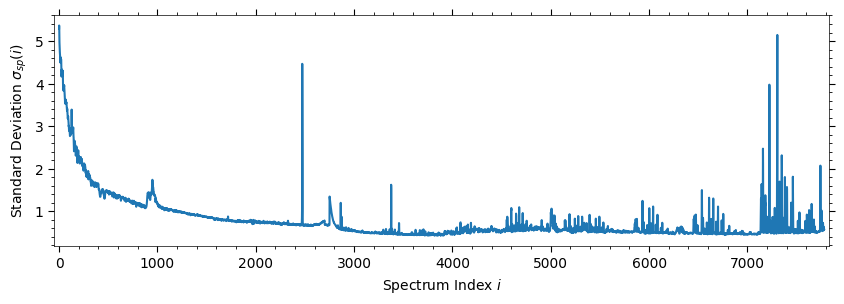
\includegraphics[width=1\textwidth]{figures/observed_spectra_std_dev}}
    \caption{$\sigma_{sp}(\lambda)$ for the training set.
    Each spectrum had 7781 bins, the x-axis represents the bin index, and the y-axis represents the standard deviation
    of the standardised bin value across all 158,377 training spectra, for that given bin.}
    \label{fig:spectra_std}
\end{figure}
$\sigma_{sp}(\lambda)$ was computed for the training set such that $\sigma_{sp}(i)$ $(i \in [0, 7781])$ gave the standard
deviation of all 158,377 train spectra measurements at the $i^{th}$ bin.
This computed $\sigma_{sp}(\lambda)$ is shown in Figure~\eqref{fig:spectra_std}.
This was useful as it meant that the noise added to the spectra at any given wavelength was proportional to the variance
of the spectra at the given wavelength, which complemented the fact that some wavelengths naturally had more variance than others,
as shown by Figure~\eqref{fig:spectra_std}.
$\gamma$ was set to 0.3.

\subsection{Redshift measurements}\label{subsec:redshift}
The redshift measurements utilised were the catalog-reported measurements and were compiled and provided directly with the
dataset by~\cite{astroclip}.

\subsection{Further Pre-processing}\label{subsec:pre-processing}
The data was pre-processed further to remove outliers and ensure data was sensible to improve training dynamics.
We dropped any galaxies with a redshift outside the range $[0, 0.8]$ and also dropped any galaxies which had every element
in their spectra equal to 0 (given that they were clearly erroneous).
This resulted in removing a further 1,508 samples from the training dataset and 380 samples from the
validation set.
Our redshift range of $[0, 0.8]$ was larger than the range of $[0, 0.6]$ used by~\cite{astroclip} in their final results.
